%!TEX root = ../Thesis.tex
\lstset {language=C++}

\chapter{VRInteractions}
\lhead{\emph{VRInteractions}}
In dit hoofdstuk worden de keuzes voor en de werking van de VRInteractions \gls{ue4} plugin besproken. 
Voor elk component in de plugin word de werking en mogelijkheden getoond. Daarnaast word voor elk component, waar relevant, besproken hoe de workshops de design keuzes beïnvloed heeft.

\section{De plugin}
De VRInteractions plugin is een combinatie van c++ code, Blueprints en overschrijfbare game modes.
De plugin heeft als doel om de \gls{vr} specifieke logica te verbergen voor gameplay logica zodat niet-programmeurs interactieve \gls{vr} omgevingen kunnen maken.

De plugin word ontwikkeld volgens de workflow die beschreven word in Hoofdstuk~\ref{ch:BlueprintsEnCpp} op pagina~\pageref{ch:BlueprintsEnCpp}.

De plugin bevat op moment van schrijven de volgende componenten:
\begin{itemize}
	\item Gamemodes
		\begin{itemize}
			\item VRInteractionsFlyTroughGameMode
			\item VRInteractionsGameMode
		\end{itemize}
	\item Characters
		\begin{itemize}
			\item VRInteractionBaseCharacter
			\item VRInteractionCharacter
			\item VRInteractionsFlyCharacter
		\end{itemize}
	\item VRInteractionsPlayerController
	\item VRInteractionsCameraManager
	\item VRInteractionsHud
	\item LookEventsComponent
	\item CircleMenu
	\item VRMovableMesh
\end{itemize}

\section{Gamemodes}
De plugin bevat de game modes VRInteractionsFlyTroughGameMode en VRInteractionsGameMode. Deze modes zijn beide een uitbreiding van de voorbeeld \gls{ue4} characters. Beide gamemodes zijn geschikt voor zowel de Oculus als de GearVR. 

De game modes zijn bedoelt om de basis instellingen voor \gls{vr} in te stellen en zijn voor de meeste applicaties voldoende. In het geval dat er iets in de gamemode aangepast moet worden is het mogelijk de instelling te overschrijven of de gehele gamemode over te erven.

Omdat er gebruik word gemaakt van een aantal input events is het aan te raden om een project altijd te beginnen als First Person Template.

\subsection{VRInteractionsGameMode}
De VRInteractionsGameMode maakt gebruik van de VRInteractionCharacter, VRInteractionsHud, VRInteractionsPlayerController en de VRInteractionsCameraManager. 

De game mode is bedoeld voor spellen waarin de speler kan rondlopen en zorgt ervoor dat de headset juist word geïnstalleerd en de juiste controllers ingesteld staan.

\subsection{VRInteractionsFlyTroughGameMode}
De VRInteractionsFlyTroughGameMode is een gestripte versie van de VRInteractionsGameMode en maakt gebruik van de VRInteractionsFlyCharacter, VRInteractionsHud, VRInteractionsPlayerController en VRInteractionsCameraManager.

Deze gamemode is bedoelt voor VR projecten waarin de speler door behulp van Matinee rondvliegt.

\section{Characters}
De VRInteractionsCharacters bevatten alle beweging en camera instellingen zoals oog hoogte. De instelling zijn gebaseerd op de \gls{vr} guidelines van Epic \href{https://docs.unrealengine.com/latest/INT/Platforms/VR/ContentSetup/index.html#vrcharactersettings}{https://docs.unrealengine.com/latest/INT/Platforms/VR/ContentSetup/index.html}.

\subsection{VRInteractionBaseCharacter}
De VRInteractionBaseCharacter is de basis voor de VRInteractionCharacter en de VRInteractionsFlyCharacter. Deze character bevat de instellingen voor de camera hoogte en wat \gls{vr} gerelateerde logica zoals het roteren van de speler op basis van zijn kijk richting.

Ook word hierin de GearVR touch pad input afgehandeld.

Het is niet de bedoeling deze classe direct te implementeren. In plaats daarvan kan er gekozen worden voor de VRInteractionCharacter of de VRInteractionsFlyCharacter. Als er een nieuwe soort character gemaakt moet worden kan die natuurlijk overerven van de VRInteractionBaseCharacter.

\subsection{VRInteractionCharacter}
De VRInteractionCharacter is bedoelt voor spellen waarin de speler rond kan lopen. De instellingen en functies zijn op basis van de \gls{ue4} \gls{vr} guidelines en de testen van de \gls{vr} demo gemaakt.

\subsection{VRInteractionsFlyCharacter}
De VRInteractionCharacter is bedoelt voor spellen waarin de speler op een rails loopt. Het is mogelijk deze character makkelijk in Matinee te gebruiken. Verschil met de VRInteractionCharacter, naast het niet registeren van controle gerelateerde input, is dat de camera niet op oog hoogte maar in het midden van de character geplaatst word. Dit maakt het maken van de Matinee sequences logischer.

\section{VRInteractionsPlayerController}
\dots

\section{VRInteractionsCameraManager}
\dots

\section{VRInteractionsHud}
De VRInteractionsHud is de basis \gls{hud} die een cirkel tekent in het midden van het scherm om aan te geven dat er naar een actor met een LookEvent gekeken word.

\begin{figure}[H]
  \centering
    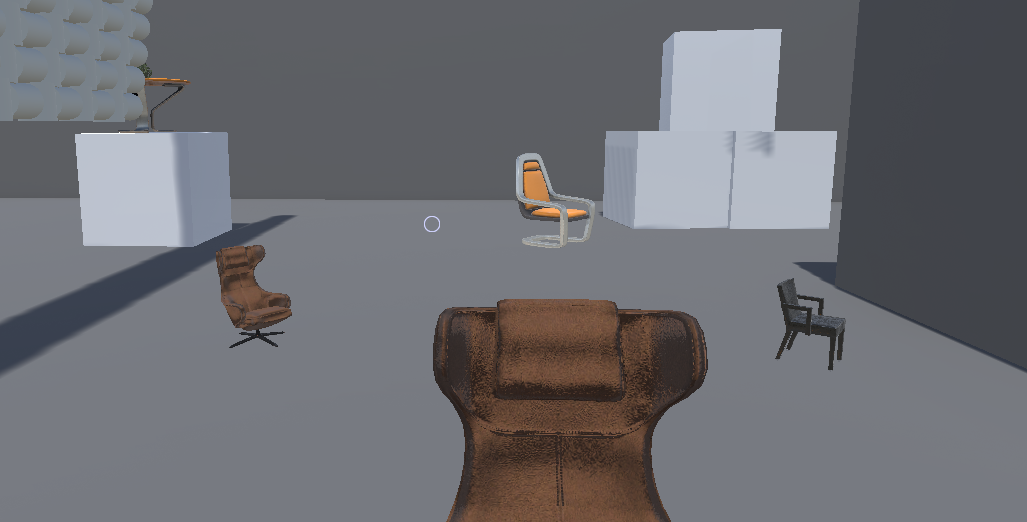
\includegraphics[width=\linewidth,height=\textheight,keepaspectratio]{HudExample}
    \caption{De cirkel die getekend word op het moment dat er naar een Actor met een LookEventsComponent gekeken word.}
\end{figure}

De \gls{hud} is afhankelijk van de VRInteractionsDataSingleton. Om te zorgen dat deze altijd correct word ingeladen kan de singleton als Game Singleton Class ingesteld worden. De singleton word namelijk gebruikt om informatie van de LookEventsComponents te verzamelen.

\section{LookEventsComponent}
\dots

\section{CircleMenu}
\dots

\section{VRMovableMesh}
\dots